\chapter{Panduan Latex}

\section{Syntax Dasar}

\subsection{Penggunaan Sitasi}
Contoh penggunaan sitasi \cite{lukito2016,santosa2011user}
\cite{setiawan2014fuzzy} \cite{wibowo2014line} \cite{marenda2016digitory} \cite{wibirama2013dual,wibowo2016clustering}

\subsection{Penulisan Gambar}

\begin{figure}[h]
	\centering
	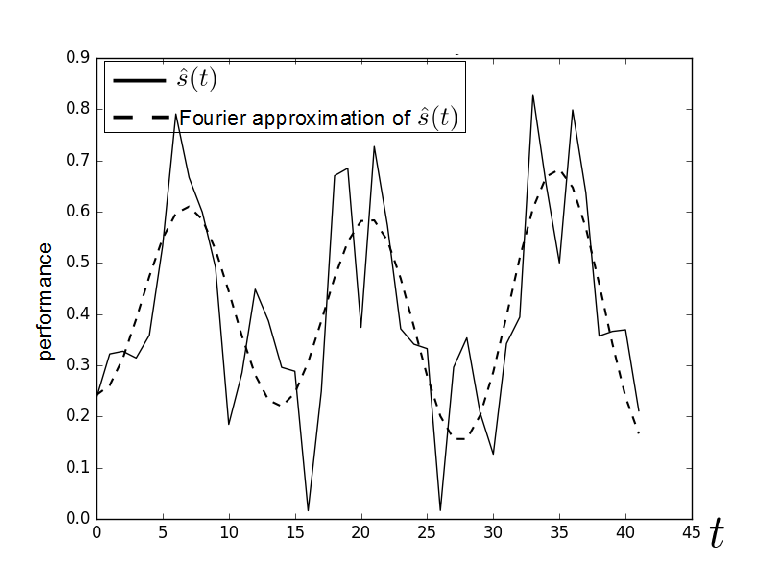
\includegraphics[width=10cm]{contents/chapter-1/sample-fig.png}
	\caption{Contoh gambar.}
	\label{Fig: Contoh gambar}
\end{figure}

Contoh gambar terlihat pada Gambar \ref{Fig: Contoh gambar}. Gambar diambil dari \cite{wibowo2016clustering}.

\subsection{Penulisan Tabel}
\begin{table}[h]
	\caption{Tabel ini}
	\vspace{0.5em}
	\centering
	\begin{tabular}{|c|c|c|}
		\hline
		ID & Tinggi Badan (cm) & Berat Badan (kg) \\
		\hline \hline
		A23 & 173 & 62 \\
		A25 & 185 & 78 \\
		A10 & 162 & 70 \\ \hline
	\end{tabular}
	\label{Tab: Tabel Tinggi Berat}
\end{table}
Contoh penulisan tabel bisa dilihat pada Tabel \ref{Tab: Tabel Tinggi Berat}.

\subsection{Penulisan formula}
Contoh penulisan formula
\begin{equation}
	L_{\psi_z} = \{ t_i \mid v_z(t_i) \le \psi_z \}
\end{equation}

Contoh penulisan secara \textit{inline}: $\mathit{PV = nRT}$. Untuk kasus-kasus tertentu, kita membutuhkan perintah "mathit" dalam penulisan formula untuk menghindari adanya jeda saat penulisan formula.

Contoh formula \textbf{tanpa} menggunakan "mathit": $PVA = RTD$

Contoh formula \textbf{dengan} menggunakan "mathit": $\mathit{PVA = RTD}$



\subsection{Contoh list}
Berikut contoh penggunaan list
\begin{enumerate}
	\item First item
	\item Second item
	\item Third item
\end{enumerate}

\section{Blok Beda Halaman}

\subsection{Membuat algoritma terpisah}

Untuk membuat algoritma terpisah seperti pada contoh berikut, kita dapat memanfaatkan perintah \textit{algstore} dan \textit{algrestore} yang terdapat pada paket \textit{algcompatible}. Pada dasarnya, kita membuat dua blok algoritma dimana blok pertama kita simpan menggunakan \textit{algstore} dan kemudian di-restore menggunakan \textit{algrestore} pada algoritma kedua. Perintah tersebut dimaksudkan agar terdapat kesinamungan antara kedua blok yang sejatinya adalah satu blok. 

\begin{algorithm}                     
	\caption{Contoh algorima}          
	\label{findme}                          
	\begin{algorithmic} [1]                   
		\Procedure{CreateSet}{$v$}
		\State Create new set containing $v$
		\EndProcedure
		\algstore{myalg}
	\end{algorithmic}
\end{algorithm}

Pada blok algoritma kedua, tidak perlu ditambahkan caption dan label, karena sudah menjadi satu bagian dalam blok pertama. Pembagian algoritma menjadi dua bagian ini berguna jika kita ingin menjelaskan bagian-bagian dari sebuah algoritma, maupun untuk memisah algoritma panjang dalam beberapa halaman.

\begin{algorithm}                     
	\begin{algorithmic} [1]                   
		\algrestore{myalg}
		\Procedure{ConcatSet}{$v$}
		\State Create new set containing $v$
		\EndProcedure
	\end{algorithmic}
\end{algorithm}


\subsection{Membuat tabel terpisah}

Untuk membuat tabel panjang yang melebihi satu halaman, kita dapat mengganti kombinasi \textit{table + tabular} menjadi \textit{longtable} dengan contoh sebagai berikut.

\begin{longtable}{| c | c |} 
	\caption{Contoh tabel panjang}
	\label{tab:myfirstlongtable} \\
	\hline
	header 1 & header 2 \\
	\hline \hline
	foo & bar \\ \hline 
	foo & bar \\ \hline
	foo & bar \\ \hline
	foo & bar \\ \hline
	foo & bar \\ \hline
	foo & bar \\ \hline
	foo & bar \\ \hline
	foo & bar \\ \hline
	foo & bar \\ \hline
	foo & bar \\ \hline
	foo & bar \\ \hline
\end{longtable}


\subsection{Menulis formula terpisah halaman}

Terkadang kita butuh untuk menuliskan rangkaian formula dalam jumlah besar sehingga melewati batas satu halaman. Solusi yang digunakan bisa saja dengan memindahkan satu blok formula tersebut pada halaman yang baru atau memisah rangkaian formula menjadi dua bagian untuk masing-masing halaman. Cara yang pertama mungkin akan menghasilkan alur yang berbeda karena ruang kosong pada halaman pertama akan diisi oleh teks selanjutnya. Sehingga di sini kita dapat memanfaatkan \textit{align} yang sudah diatur dengan mode \textit{allowdisplaybreaks}. Penggunakan \textit{align} ini memungkinkan satu rangkaian formula terpisah berbeda halaman. 

Contoh sederhana dapat digambarkan sebagai berikut.

\begin{align*}
	x &= y^2\\
	x &= y^3\\
	a + b &= c\\
	x &= y - 2\\
	a + b &= d + e \tag{\stepcounter{equation}\theequation}\\
	x^2 + 3 &= y\\
	a(x) &= 2x\\
	b_i &= 5x\\
	10x^2 &= 9x\\
	2x^2 + 3x + 2 &= 0\\
	5x - 2 &= 0\\
	d &= \log x\\
	y &= \sin x
\end{align*}

